
\chapter{Resultados y pruebas}

En las siguientes secciones se expondrán los resultados que se han obtenido tras usar la nueva nomenclatura implementada y los cambios en el sistema de representación. Se describirán también las pruebas llevadas a cabo para validar todo este proceso.

\section{Nomenclatura canónica}
- Poner una tabla con las moléculas: smiles original, dibujo original, smiles canonico, dibujo canonico (a ser posible mejorado)

\textbf{Para los resultados de la canonizacion tendré que hacer una tabla comparando ambas cadenas o algo asi}

Con esta solución en donde se organiza el SMILES según sus ramificaciones, se ha intentado también dar un enfoque al canonizado orientado a la representación 2D. De esta manera, podemos visualizar ambos e identificar claramente la correspondencia entre una porción del SMILES con una sección de la representación. Así, se recorren primero todos los vecinos de un átomo hasta cerrar esa rama antes de pasar a la siguiente, obteniendo un SMILES más limpio. (ilustrar esto con una imagen que me invente yo). Se ilustra esto en las siguientes Figuras \ref{fig:smiles_vs_dibujo}.
auqi puedo usar la mol 24, la 23, o la 5 simetrica, o alguna de las ultimas de iridio.

\begin{figure}[h!]
    \centering
    
\includegraphics[scale=0.5]{imagenes/placeholder.png}
    \caption{Correspondencia entre el SMILES canónico y la representación 2D de la molécula.}
    \label{fig:smiles_vs_dibujo}
\end{figure}

\section{Sistema de representación 2D}

\textbf{PH}(aqui tengo que mostrar 100\% la evolución de 2 o 3 para el ironII, para ilustrar este proceso de pensado que explico. Luego ya en resultados muestro todas en sus versiones finales). 


Los ficheros svg completos con el antes y el después para el conjunto de datos que he usado están disponibles para su consulta en GitHub.

Meter una evolución de 3 fotos del progreso del dibujado. Y poner algo tipo “Se han alcanzado varios modos de dibujado pero el experto finalmente ha preferido el X, por ser el más comodo y entendible entre químicos y ser más utilizado en la literatura” (siguiendo además el manual mencioando en la seccion \ref{implementacion:dibujado} anteriormente). Puedo tener un par de moléculas de juguete/referencia en donde voy mostrando los cambios gordos que voy aplicando; y luego la tabla grande con todo el dataset (cuando ejecuto todas juntas) como para mostrar el “antes mal -> ahora bien”. Aquellas que tanto antes como después las dibuje bien o igual, puedo poner una o un par y listo (no todas).

(siguiendo el este estándar de la iupac mencionado en la Sección \ref{implementacion:dibujado}, las líneas gordas son preferibles. Pero para moléculas de este tipo donde todo sale muy pegado, y según las recomendaciones de los expertos es mejor que salga todo un poco más espaciado. Si bien esto no arregla el solapamiento (esto requiere de un cambio sustancial en el algoritmo de generación de coordenadas), mejora minimante la visibilidad de los enlaces)

Poner tambien las versiones sin alias y con alias. “version sin alias vs version con alias, puede quedar más legible”, “la visualización se puede mejorar aun, utilizando la opción de generación de abreviaturas de OpenBabel”, con los parámetros --genalias -xA en la línea de ordenes, podemos invocar esta funcionalidad. Esto consiste en “… blah blah, fichero de base de datos, equivalencias, no se que”

Mostrar tb el dubujo del rutenio ultimo, para mostrar que se detectan no solo Cp de 5, sino de más carbonos tambien.

\section{Pruebas}
El propio proyecto de OpenBabel ya trae consigo un entorno de pruebas, que se gestiona a través del ejecutable 'test\_runner.exe'. Según los parámetros que le pases al programa, se ejecutará un test u otro. Dichos tests pueden incluso albergar otros tests más específicos dentro. La ejecución de un test concreto sigue este esquema: 
\begin{center}
    \textit{test\textunderscore runner \textless nombreTest\textgreater  \textless numeroTest\textgreater}    
\end{center}

Un ejemplo de llamada al test ``conversion", que es un test único sería: \textit{test\_runner.exe conversion}. Con la llamada \textit{test\_runner.exe regressiontest 225} se estaría ejecutando el test número 225 especificado en regressiontest.cpp. A la hora de añadir nuevos ficheros de testing hay que seguir una serie de indicaciones y utilizar una sintaxis especial para determinar si el test es correcto o no. Esto se describe en la guía para desarrolladores de la página oficial de OpenBabel\footnote{\url{https://openbabel.org/docs/current/Contributing/Testing.html}}\footnotecomma\footnote{\url{https://open-babel.readthedocs.io/en/latest/Contributing/Testing.html}} (en el Anexo \ref{apend:manual} se describe como añadir nuevos tests).

Dicho esto, la mayoría de tests que se han realizado son tests funcionales completos. Hacer un test de unidad de según que métodos es complicado ya que necesitan una serie de parámetros y variables que se van creando sobre la marcha en multitud de métodos previos. El fichero de pruebas creado específicamente para el proyecto se llama ``canonogmtest.cpp'' y tiene la siguiente estructura:
\textbf{METER un salto de pagina por si queda mal del dirtree al acabar todo}
\vspace{0.2cm}
\dirtree{%
    .1 test\_runner.cpp\DTcomment{fichero main gestor de pruebas}.
    .2 canonogmtest.cpp\DTcomment{fichero main de pruebas para el proyecto}.
    .3 SelectCanonMetal\DTcomment{prueba 1}.
    .3 RandomCanonStandardLabels\DTcomment{prueba 2}.
    .3 RandomCanonCanonicalLabels\DTcomment{prueba 3}.
    .3 CanonOverCanon\DTcomment{prueba 4}.
    .3 DrawDoubleCpTest\DTcomment{prueba 5}.
    .2 Otros .cpp de pruebas creados por OpenBabel.
    .3 regressiontest.cpp.
    .3 ringtest.cpp.
    .3 invalidsmiles.cpp.
    .3 conversion.cpp.
    .3 ....
    .3 ....
}

En el GitHub del proyecto se pueden consultar los ficheros de salida que resultaron de la ejecución de las pruebas (las que tengan alguna salida).\textbf{AÑADIR ESTO A GITHUB} Este proceso de testing, tal como indico en la Sección \ref{aplicacion_metod}, se realizaba de manera frecuente para comprobar si los resultados iban siendo los esperados. A continuación se describen las pruebas llevadas a cabo:

\begin{itemize}
    \item \textbf{Test unitario}
    \begin{itemize}
        \item \textbf{SelectCanonMetal}: comprueba que el método \textit{OBMol2Cansmi:: SelectRootAtomOgm} funciona correctamente eligiendo el átomo adecuado de entre todos los átomos para moléculas que contengan algún metal. Los SMILES a comprobar se cargan de un fichero, junto con el identificador del átomo que se debería seleccionar. El test es válido si el identificador cargado y el que devuelve el método coinciden.
    \end{itemize}

    \item \textbf{Tests funcionales}
    \begin{itemize}
        \item \textbf{RandomCanonStandardLabels}: comprueba la consistencia de la nomenclatura canónica para la forma estándar. Se toman los SMILES de prueba desde un fichero y se obtienen unos SMILES sinónimos de manera aleatoria para la misma molécula. Tanto el SMILES original como el randomizado se canonizan a su forma estándar. El test es válido si ambos canónicos obtenidos coinciden. Por lo general, teniendo en cuenta lo discutido en la Sección \ref{implementacion:canonizado} es normal que el test falle.

        \item \textbf{RandomCanonCanonicalLabels}: comprueba la consistencia de la nomenclatura canónica para la forma canónica. Se toman los SMILES de prueba desde un fichero y se obtienen unos SMILES sinónimos de manera aleatoria para la misma molécula. Tanto el SMILES original como el randomizado se canonizan a su forma canónica. El test es válido si ambos canónicos obtenidos coinciden.
    
        \item \textbf{CanonOverCanon}: comprueba la consistencia de la nomenclatura canónica. Se toman los SMILES de prueba desde un fichero y se canonizan. A esos SMILES canonizados, se les vuelve a aplicar el algoritmo. Con este test se quiere verificar que sucesivas aplicaciones del algoritmo no degeneren el resultado o haya una vaivén de los átomos, como sería el caso de la Figura \ref{fig:canonOverCanon}. El test es válido si ambos resultados coinciden.

        \begin{figure}[h!]
            \centering
            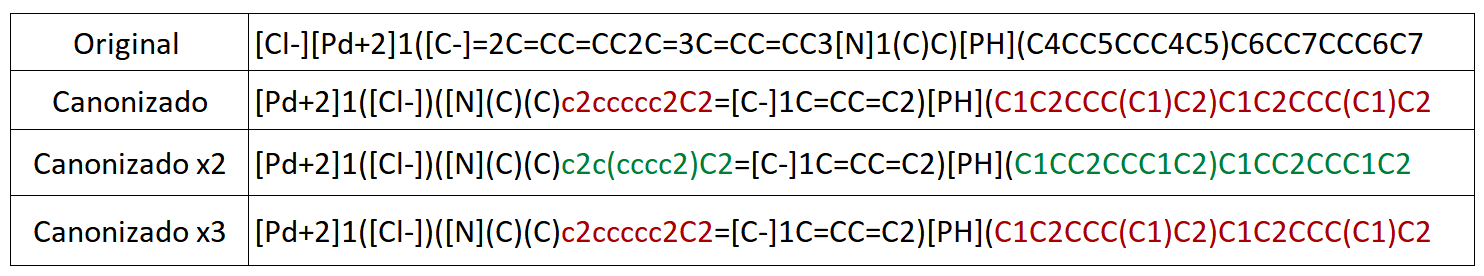
\includegraphics[scale=0.3]{imagenes/resultados/pruebas/canonOverCanon.png}
            \caption{Ejemplo de una canonización imperfecta. Se muestra el SMILES original, y los SMILES canónicos tras haber aplicado 1, 2 y 3 veces el algoritmo sobre el anterior resultado respectivamente. Esto no ocurre con ninguna de las moléculas probadas.}
            \label{fig:canonOverCanon}
        \end{figure}
    
        \item \textbf{DrawDoubleCpTest}: comprueba si los algoritmos de dibujado para moléculas con múltiples Cp se aplican correctamente. Se introduce una molécula sabida de antemano que contiene varias de estas estructuras y se realiza la conversión. El test en sí tiene es válido si el proceso de conversión tiene éxito. Dado que analizar de manera automática el resultado de una representación gráfica en formato .svg no es tarea fácil, hay que verificar si el resultado es el esperado de acuerdo a lo descrito en la Sección \ref{implementacion:dibujado} de manera manual.
    
    \end{itemize}
\end{itemize}

Se han ejecutado también otros tests útiles como el \textit{invalidsmiles} para comprobar que OpenBabel rechazaba SMILES incorrectos. Decir que para los tests \textit{RandomCanonStandardLabels}, \textit{RandomCanonCanonicalLabels} y \textit{CanonOverCanon} se han usado datasets relativamente grandes, de aproximadamente 1000 moléculas incluyendo química orgánica general y las moléculas nuestras propias de organometálica. Para todas ellas, salvo 6 excepciones de estereoquímica con compuestos cis/trans, el test se cumple. Las otras dos pruebas son mucho más selectivas y específicas, por lo que se han aplicado a nuestro dataset simplemente.

